\section{Results}
\label{sec:results}
The results are presented in the order of the argument: the pre-fit gate, the accuracy of the expanded arms against cohort whitening and the random control, the profile over the added trace $s$, and the diagnostics that relate accuracy to the captured span.

\subsection{Pre-fit gate}
\label{sec:gate-results}
The within-patient complement locates the missing span well on both datasets, and the gate passed by a wide margin (Table~\ref{tab:gate}). On TCGA-UT its leading $r_B=120$ directions hold 14.2 percent of the pool's between-patient variance at five patients, against 20.3 percent for the best 120-dimensional subspace of the complement and 1.5 percent for 120 random complement directions, so the gate fraction is 0.68. The fraction rises with $k$ and reaches 0.93 at $k=8r_B=960$, where the within-patient directions hold 28.5 of the 30.2 percent that lies outside the cohort basis at all. On BRACS the fraction is lower, 0.56 at $k=r_B=28$ and 0.73 at $k=8r_B$, but it is still far above the stopping threshold of 0.1. The numbers are internally consistent: the oracle share never exceeds the complement's share of the pool variance, and the within-patient share lies between the random and the oracle share at every $k$.

\begin{table}[htbp]
\centering
\small
\renewcommand{\arraystretch}{1.15}
\begin{tabular}{@{}lrrrrrrrr@{}}
\toprule
 & \multicolumn{4}{c}{TCGA-UT, $r_B=120$} & \multicolumn{4}{c}{BRACS, $r_B=28$} \\
\cmidrule(lr){2-5}\cmidrule(lr){6-9}
 & $k=r_B$ & $2r_B$ & $4r_B$ & $8r_B$ & $k=r_B$ & $2r_B$ & $4r_B$ & $8r_B$ \\
\midrule
Within-patient complement & 0.142 & 0.196 & 0.245 & 0.285 & 0.158 & 0.213 & 0.267 & 0.317 \\
Random complement & 0.015 & 0.030 & 0.059 & 0.118 & 0.005 & 0.009 & 0.019 & 0.037 \\
Best complement subspace & 0.203 & 0.249 & 0.281 & 0.298 & 0.279 & 0.348 & 0.398 & 0.420 \\
\addlinespace
Gate fraction $f$ & 0.68 & 0.76 & 0.84 & 0.93 & 0.56 & 0.60 & 0.66 & 0.73 \\
\bottomrule
\end{tabular}
\caption{The within-patient complement finds most of the pool's between-patient variance that the cohort basis misses. Entries are shares of the pool's between-patient variance in the span of the first $k$ complement directions, at five patients per class, averaged over ten draws of split 0; the gate fraction is $(W-\text{random})/(\text{oracle}-\text{random})$, averaged per draw. The cohort basis itself holds 0.698 (TCGA-UT) and 0.577 (BRACS) of the pool variance \citep{queisler2026spectrumRegularization}.}
\label{tab:gate}
\end{table}

\subsection{Accuracy against cohort whitening}
\label{sec:accuracy-results}
The expanded arm fails the prespecified criterion on both datasets. On TCGA-UT the tuned arm gains 0.45 points over cohort whitening at five patients per class (0.27 to 0.63), so the interval lies above zero but the estimate falls short of the one-point threshold (Table~\ref{tab:accuracy}). On BRACS the gain has the same point estimate, 0.45 points, but its interval runs from $-0.35$ to 1.21. The gain shrinks with the patient count: on TCGA-UT it is 0.06 points at ten patients ($-0.05$ to 0.19) and 0.00 at twenty ($-0.03$ to 0.03), and on BRACS 0.29 ($-0.19$ to 0.90) and $-0.03$ ($-0.46$ to 0.39).

\begin{table}[htbp]
\centering
\small
\renewcommand{\arraystretch}{1.15}
\begin{tabular}{@{}lrrr@{}}
\toprule
Arm family & $G=5$ & $G=10$ & $G=20$ \\
\midrule
\multicolumn{4}{@{}l}{\emph{TCGA-UT}}\\
Real cohort (R) & 62.48 [61.24, 63.65] & 67.79 [66.47, 69.00] & 71.89 [70.55, 73.06] \\
Cohort whitening, $s=0$ (RWc) & 64.74 [63.52, 65.90] & 69.64 [68.34, 70.84] & 73.16 [71.86, 74.34] \\
$s=0.1$ (Wa) & 65.01 [63.79, 66.16] & 69.69 [68.40, 70.88] & 73.17 [71.87, 74.35] \\
$s=0.3$ (Wb) & 65.25 [64.02, 66.40] & 69.71 [68.41, 70.86] & 73.17 [71.87, 74.34] \\
$s=1$ (Wc) & 65.16 [63.91, 66.32] & 69.65 [68.37, 70.85] & 73.15 [71.84, 74.31] \\
$s=3$ (Wd) & 64.77 [63.50, 65.93] & 69.50 [68.22, 70.72] & 73.09 [71.79, 74.26] \\
Tuned $s$ (Wt) & 65.19 [63.95, 66.34] & 69.71 [68.42, 70.89] & 73.16 [71.87, 74.33] \\
Random complement, tuned $s$ (Rt) & 64.77 [63.54, 65.93] & 69.65 [68.33, 70.83] & 73.15 [71.85, 74.33] \\
Pool-basis whitening (RW) & 67.40 [66.14, 68.52] & 71.66 [70.39, 72.84] & 74.44 [73.10, 75.59] \\
Pool centres (C) & 73.14 [71.62, 74.50] & 74.47 [73.01, 75.78] & 75.55 [74.11, 76.85] \\
\addlinespace
Gain Wt $-$ RWc & \textbf{0.45} [0.27, 0.63] & 0.06 [$-$0.05, 0.19] & 0.00 [$-$0.03, 0.03] \\
Gain Wt $-$ Rt & 0.42 [0.25, 0.60] & 0.06 [$-$0.05, 0.18] & 0.01 [$-$0.02, 0.03] \\
Gain Rt $-$ RWc & 0.02 [$-$0.01, 0.06] & 0.00 [$-$0.01, 0.01] & $-$0.01 [$-$0.02, 0.01] \\
Gain Wt $-$ R & 2.71 [2.35, 3.04] & 1.92 [1.62, 2.20] & 1.27 [1.04, 1.50] \\
\addlinespace
\multicolumn{4}{@{}l}{\emph{BRACS}}\\
Real cohort (R) & 36.18 [33.46, 38.80] & 38.49 [35.87, 41.22] & 40.97 [38.50, 43.62] \\
Cohort whitening, $s=0$ (RWc) & 36.49 [33.87, 39.24] & 38.61 [35.94, 41.34] & 41.28 [38.70, 43.88] \\
$s=0.1$ (Wa) & 37.09 [34.47, 39.70] & 38.69 [36.03, 41.43] & 41.20 [38.64, 43.74] \\
$s=0.3$ (Wb) & 37.14 [34.59, 39.70] & 39.02 [36.33, 41.65] & 41.32 [38.77, 43.89] \\
$s=1$ (Wc) & 36.91 [34.28, 39.52] & 38.99 [36.32, 41.65] & 41.24 [38.73, 43.78] \\
$s=3$ (Wd) & 36.77 [34.14, 39.35] & 38.80 [36.19, 41.42] & 41.26 [38.77, 43.78] \\
Tuned $s$ (Wt) & 36.94 [34.39, 39.48] & 38.90 [36.30, 41.53] & 41.26 [38.76, 43.77] \\
Random complement, tuned $s$ (Rt) & 36.56 [33.91, 39.27] & 38.65 [35.96, 41.40] & 41.26 [38.72, 43.81] \\
Pool-basis whitening (RW) & 39.50 [36.82, 41.98] & 40.13 [37.39, 42.77] & 41.25 [38.79, 43.76] \\
Pool centres (C) & 44.63 [41.33, 48.05] & 45.11 [41.85, 48.51] & 45.50 [42.20, 48.76] \\
\addlinespace
Gain Wt $-$ RWc & \textbf{0.45} [$-$0.35, 1.21] & 0.29 [$-$0.19, 0.90] & $-$0.03 [$-$0.46, 0.39] \\
Gain Wt $-$ Rt & 0.38 [$-$0.42, 1.16] & 0.25 [$-$0.24, 0.86] & $-$0.01 [$-$0.37, 0.44] \\
Gain Rt $-$ RWc & 0.06 [$-$0.03, 0.26] & 0.04 [$-$0.04, 0.16] & $-$0.02 [$-$0.28, 0.14] \\
Gain Wt $-$ R & 0.77 [$-$0.16, 1.72] & 0.40 [$-$0.24, 1.13] & 0.28 [$-$0.49, 1.15] \\
\bottomrule
\end{tabular}
\caption{Adding the within-patient complement to cohort whitening gains about half a point at five patients and nothing at twenty; the same eigenvalues on random directions gain nothing. Accuracy entries are test patient-macro balanced accuracy in percent; gains are paired contrasts in percentage points; bold entries are the primary contrast. Intervals are 95\% bootstrap intervals over test patients and draws. The R, C, RWc, and RW rows are the fits of \citet{queisler2026centreError}, \citet{queisler2026patientDirections}, and \citet{queisler2026bracsMechanism}.}
\label{tab:accuracy}
\end{table}

\noindent The gain on TCGA-UT is specific to the within-patient directions. The tuned random control gains 0.02 points over cohort whitening at five patients ($-0.01$ to 0.06), and the specificity contrast Wt5$-$Rt5 is 0.42 points (0.25 to 0.60). Every fixed-$s$ random arm stays within 0.04 points of cohort whitening at every patient count on TCGA-UT and within 0.07 points on BRACS; only two of these 24 contrasts have an interval that excludes zero, both small and negative: Rc10 and Rd10 on TCGA-UT at $-0.01$ ($-0.02$ to $-0.00$) and $-0.04$ points ($-0.09$ to $-0.01$). Contracting random directions of the complement therefore neither helps nor hurts by more than a few hundredths of a point. On BRACS the specificity contrast is 0.38 points ($-0.42$ to 1.16), in the same direction as on TCGA-UT but not resolved.

Measured against the gap it was meant to close, the gain is small. At five TCGA-UT patients the tuned arm closes a share of 0.169 (0.105 to 0.231) of the 2.66-point gap between cohort-basis and pool-basis whitening, and 0.032 ($-0.024$ to 0.089) of the 2.02-point gap at ten patients. Its recovery of the pool-centre headroom is 0.254 (0.221 to 0.289) at five patients and 0.287 (0.241 to 0.337) at ten, against 0.212 and 0.277 for cohort whitening. Because the gain is concentrated at five patients, it also narrows the patient-count gap: the tuned arm removes a share of 0.153 (0.119 to 0.185) of the 9.41-point gap between five and twenty patients, that is 1.44 points, against 0.105 (0.074 to 0.136) or 0.99 points for cohort whitening. On BRACS the headroom share is 0.149 ($-0.140$ to 0.391) of a 3.01-point gap at five patients, and the recovery of 0.091 ($-0.020$ to 0.196) is indistinguishable from zero.

\subsection{The profile over the added trace}
\label{sec:profile-results}
At five TCGA-UT patients the gain has an interior maximum in $s$ (Figure~\ref{fig:profile}). It is 0.26 points at $s=0.1$ (0.14 to 0.40), 0.51 at $s=0.3$ (0.33 to 0.68), 0.42 at $s=1$ (0.21 to 0.63), and 0.02 at $s=3$ ($-0.17$ to 0.23). The tuned arm, at 0.45 points, reaches nearly the best fixed value, so validation selection loses little. At ten and twenty patients no fixed $s$ gains more than 0.06 points, and the largest added trace becomes harmful: $s=3$ costs 0.14 points at ten patients ($-0.27$ to 0.00) and 0.07 at twenty ($-0.12$ to $-0.02$). The random arms are flat at zero across the whole grid.

\begin{figure}[htbp]
\centering
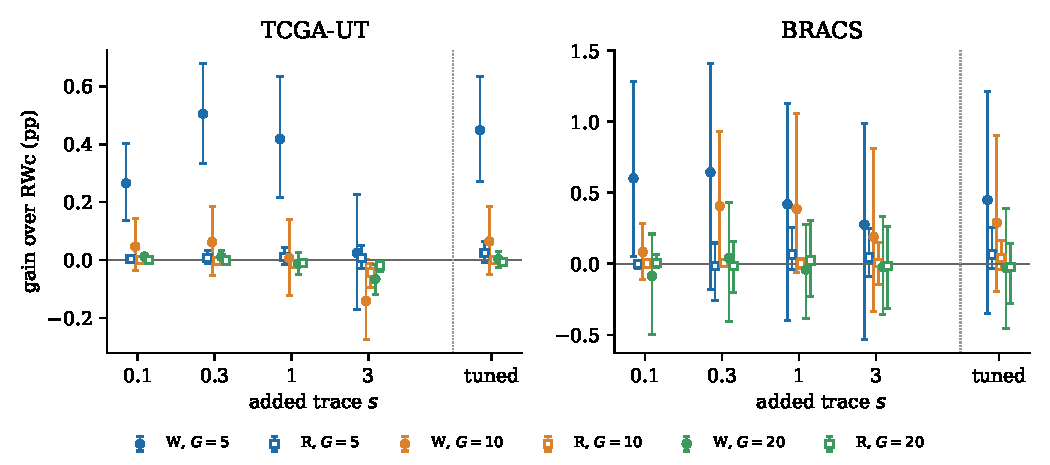
\includegraphics[width=\textwidth]{s_profile.pdf}
\caption{Within-patient directions help at five patients with an interior optimum near $s=0.3$; the same eigenvalues on random directions do nothing at any $s$. Paired gain over cohort whitening in percentage points against the added trace $s$, as a fraction of the between-patient trace; $s=0$ is cohort whitening and therefore zero by construction. Filled circles are the within-patient arms W, open squares the random-complement control R, and the markers right of the dotted line are the validation-tuned arms. Error bars show the paired 95\% bootstrap intervals; markers are offset horizontally to separate patient counts and families.}
\label{fig:profile}
\end{figure}

\noindent The BRACS profile has the same shape at five patients but much wider intervals. Only the smallest added trace has an interval that lies above zero, 0.60 points at $s=0.1$ (0.05 to 1.28); the peak estimate is 0.64 at $s=0.3$ ($-0.18$ to 1.41). This is one of twelve fixed-$s$ contrasts on BRACS and not the primary contrast, so it does not establish a gain on that dataset. At ten patients the estimates are 0.08 to 0.41 points with intervals that include zero, and at twenty they are within 0.09 points of zero.

\subsection{Diagnostics and validation selection}
\label{sec:diagnostics-results}
The selected expanded covariances capture much more of the pool's between-patient variance than the cohort basis does, and far more than the random control (Table~\ref{tab:diagnostics}). At five TCGA-UT patients, the top $r_B$ eigenvectors of the selected $\hat{\boldsymbol\Sigma}_s$ capture 0.711 of the pool variance and the top $8r_B$ capture 0.977, against 0.698 for the cohort basis alone and 0.795 for the random control at $8r_B$. On BRACS the corresponding values are 0.583 and 0.866, against 0.577 and 0.607. The first $r_B$ added directions overlap the pool's top $r_B$ directions by 0.27 on TCGA-UT and 0.19 to 0.22 on BRACS, five to twenty times the value $r_B/2{,}560$ of an unrelated subspace at five patients.

\begin{table}[htbp]
\centering
\small
\renewcommand{\arraystretch}{1.15}
\begin{tabular}{@{}lrrrrrr@{}}
\toprule
 & \multicolumn{3}{c}{TCGA-UT} & \multicolumn{3}{c}{BRACS} \\
\cmidrule(lr){2-4}\cmidrule(lr){5-7}
 & $G=5$ & $G=10$ & $G=20$ & $G=5$ & $G=10$ & $G=20$ \\
\midrule
Rank $r_B=C(G-1)$ & 120 & 270 & 570 & 28 & 63 & 133 \\
Captured share, cohort basis & 0.698 & 0.845 & 0.938 & 0.577 & 0.760 & 0.876 \\
Captured share, Wt, $k=r_B$ & 0.711 & 0.842 & 0.911 & 0.583 & 0.737 & 0.844 \\
Captured share, Wt, $k=8r_B$ & 0.977 & 0.969 & 0.996 & 0.866 & 0.911 & 0.961 \\
Captured share, Rt, $k=8r_B$ & 0.795 & 0.926 & 0.985 & 0.607 & 0.798 & 0.912 \\
Added overlap with pool basis & 0.270 & 0.265 & 0.256 & 0.221 & 0.196 & 0.189 \\
Overlap of a random subspace & 0.047 & 0.105 & 0.223 & 0.011 & 0.025 & 0.052 \\
Correlation with gain, $k=r_B$ & 0.35 & 0.15 & 0.33 & 0.37 & 0.08 & $-$0.12 \\
Correlation with gain, $k=8r_B$ & 0.31 & 0.13 & 0.01 & 0.10 & 0.15 & $-$0.05 \\
\addlinespace
Selected $s=0$ & 0 & 6 & 2 & 2 & 7 & 7 \\
Selected $s=0.1$ & 3 & 5 & 8 & 2 & 5 & 1 \\
Selected $s=0.3$ & 12 & 10 & 9 & 7 & 3 & 8 \\
Selected $s=1$ & 13 & 8 & 8 & 6 & 5 & 8 \\
Selected $s=3$ & 2 & 1 & 3 & 13 & 10 & 6 \\
\bottomrule
\end{tabular}
\caption{The expanded covariance captures most of the pool's between-patient variance, yet per-draw capture predicts the accuracy gain only weakly. Captured shares are the pool variance in the span of the top $k$ eigenvectors of the selected covariance; the cohort-basis row is taken from \citet{queisler2026spectrumRegularization} on the same cohorts. The added overlap is that of the first $r_B$ within-patient directions with the pool's top $r_B$ directions, reported for $s=1$, and the random row is its reference value $r_B/2{,}560$. The correlation is taken across the 30 fits between the gain in captured share over the cohort basis and the test gain Wt$-$RWc. The first nine rows are means over 30 fits; the selection rows count the $s$ chosen by Wt in those 30 fits.}
\label{tab:diagnostics}
\end{table}

\noindent Capture predicts accuracy only weakly. Across the 30 fits at five TCGA-UT patients, the correlation between the gain in captured share and the accuracy gain Wt$-$RWc is 0.31 to 0.35 at every $k$, and at ten patients it is 0.12 to 0.19. With 30 fits, a correlation of 0.35 lies at the edge of conventional significance (two-sided $p\approx0.06$). At twenty patients the correlation falls to 0.01 at $k=8r_B$, where the captured share is already close to one for every fit. The random control shows the same dissociation from the other side: it raises the captured share at $8r_B$ from 0.698 to 0.795 at five TCGA-UT patients without any accuracy gain.

Validation selection on TCGA-UT is informative at five patients and diffuse beyond. The tuned arm never keeps $s=0$ at five patients and chooses $s=0.3$ or $s=1$ in 25 of 30 fits, which brackets the best fixed value. At ten and twenty patients the selections spread over the whole grid, in line with the flat profile there. The random control chooses $s=3$ in 14 of 30 fits at five TCGA-UT patients, which costs nothing because the random arms are flat. On BRACS both tuned families choose $s=3$ most often at five patients, 13 and 14 of 30 fits, even though the test profile of the within-patient arm peaks at small $s$. This mismatch is what a noisy validation signal on 24 validation patients produces.

The whitening scale shifts with the added directions. On TCGA-UT at five patients the tuned arm selects grid factor 10 in 22 of 30 fits and factor 100 in 3, whereas cohort whitening selects factor 1 in almost all fits \citep{queisler2026patientDirections}; the random control keeps factor 1 in 23 of 30. Because the factors are rescaled to act on the cohort block exactly as in cohort whitening (Section~\ref{sec:model}), a larger factor contracts both the cohort block and the added block more strongly. At ten patients the tuned arm selects factor 1 in 18 and factor 10 in 11 fits, and at twenty patients factor 1 in all 30. On BRACS the factors spread mostly from 0.1 to 10 in every family, as in the earlier BRACS studies \citep{queisler2026bracsMechanism}.

\section{Discussion}
\label{sec:discussion}
Of the three readings fixed in Section~\ref{sec:evaluation}, the results select a weak form of the first on TCGA-UT and the third in substance. The within-patient complement locates the missing span, as the gate shows, and whitening along it helps in a direction-specific way at five patients, because the random control with identical eigenvalues gains nothing. The effect is small, however: 0.45 points, a sixth of the 2.66-point gap to pool-basis whitening, below the practical threshold, and absent at ten and twenty patients. On BRACS no contrast is resolved.

The central finding is a dissociation between span and accuracy. At five TCGA-UT patients the top 960 eigenvectors of the selected expanded covariance hold 98 percent of the pool's between-patient variance, almost as much as the pool basis itself, yet the arm recovers only 17 percent of the accuracy that the pool basis delivers. Capture also predicts the per-draw gain only weakly. The captured share measures whether the between-patient variance lies in the span of the chosen directions, but the whitening in Equation~\ref{eq:whiten} acts through the weight $\nu_j$ on each direction. In the expanded arm those weights are the patch-level variances $s\tau\omega_j$, not the patient-level variances the pool basis uses. The within-patient complement ranks directions by how much patches vary within a patient. Along any single direction of this ranking, the between-patient variance is a fraction of the patch-level variance, and the class signal carried by the same direction is contracted along with the patient variation. A single scalar $s$ can trade these effects against each other only on average. This reading fits the interior optimum near $s=0.3$, the harm at $s=3$ for larger patient counts, and the stronger scale factor selected at five patients. It is an interpretation, not a tested mechanism: the arm that would test it, the expanded basis with the pool's between-patient variance attached to each added direction, was not run.

The result sharpens the conclusion of \citet{queisler2026spectrumRegularization} in one respect and qualifies it in another. That study showed that the eigenvalues within the cohort basis hardly matter and that the missing directions account for almost all of the headroom. The present study shows that the missing directions can be found from the cohort's own patches, but that finding them is not enough. Outside the cohort basis, the weight attached to each direction does matter, and the cohort has no patient-level estimate of that weight, because its $C(G-1)$ patient deviations do not reach those directions. The within-patient covariance is a proxy for direction, not for patient-level strength.

For the question of this series, what recovers the patient-shortage deficit from the cohort alone, the answer does not change. At five TCGA-UT patients, the best cohort-only whitening gains 2.71 points over the real cohort, against 2.26 for cohort whitening and 4.92 for pool-basis whitening, and it removes 15 percent of the five-to-twenty patient gap. The remaining headroom requires patient-level information along directions that the labelled cohort cannot supply. Plausible sources are unlabelled slides from further patients, related cohorts, or a population covariance carried by the feature extractor.

\section{Limitations}
\label{sec:limitations}
The study does not separate direction from weight within the complement. The expanded arms attach patch-level variances to the added directions, and the random control changes the directions while keeping those variances. An arm that keeps the within-patient directions and attaches the pool's between-patient variance along each of them, in the manner of the oracle spectrum of \citet{queisler2026spectrumRegularization}, would bound what reweighting the same directions can achieve. It was not run, so the interpretation in Section~\ref{sec:discussion} is plausible but untested.

The added trace is a single scalar, and the grid $\{0.1,0.3,1,3\}$ was fixed before fitting. A truncation of the complement to its leading directions, or a separate weight per direction, could behave differently; truncation was used only as a diagnostic. The scale factor $\kappa$ is tuned jointly with $s$, and at five TCGA-UT patients the tuned arm selects a larger factor than cohort whitening. The gain therefore reflects the joint contraction of the cohort block and the added block, not the added block alone. The random control, which uses the same anchoring and the same grid and gains nothing, excludes the reading that a stronger contraction of the cohort block alone explains the gain; cohort whitening also had factor 10 available and rarely selected it.

The gate and the captured-share diagnostic measure variance in a span, which is not the quantity the classifier uses, as the weak correlations show. The gate was computed on split 0 only. On BRACS the complement has about a thousand directions rather than the full complement, because $CG(m-1)$ is smaller than the feature dimension, and the random control spans a different subspace there than on TCGA-UT. All arms reuse the three evaluation splits of the source studies, so they share test patients with every earlier comparison in this series, and repeated use of these partitions inflates the chance that some arm appears to work by selection alone; the one BRACS contrast with an interval above zero, at $s=0.1$, is of this kind. The results are conditional on frozen Virchow2 features, multinomial logistic regression, 160 patches per class, and the two cohorts studied.
